\subsection{PRM800K}
{{\footnotesize
\noindent PRM800K is a process supervision dataset containing 800,000 step-level correctness labels for model-generated solutions to problems from the MATH dataset.


\begin{description}[labelwidth=4cm, labelsep=1em, leftmargin=4cm, itemsep=0.1em, parsep=0em]
  \item[date:] 2023-05-30
  \item[version:] 1
  \item[last\_updated:] 2023-05-30
  \item[expired:] false
  \item[valid:] yes
  \item[valid\_date:] 2023-05-30
  \item[url:] \href{https://github.com/openai/prm800k/tree/main}{https://github.com/openai/prm800k/tree/main}
  \item[doi:] 10.48550/arXiv.2305.20050
  \item[domain:]
    - Mathematics
  \item[focus:] Math reasoning generalization
  \item[keywords:]
    - calculus
    - algebra
    - number theory
    - geometry
  \item[licensing:] MIT License
  \item[task\_types:]
    - Problem solving
  \item[ai\_capability\_measured:]
    - Math reasoning and generalization
  \item[metrics:]
    - Accuracy
  \item[models:]
    - GPT-4
  \item[ml\_motif:]
    - Reasoning \& Generalization
  \item[type:] Benchmark
  \item[ml\_task:]
    - Reasoning
  \item[solutions:] 0
  \item[notes:] Math problems \& Annotated reasoning steps based off of Dan Hendrycks' MATH dataset
  \item[contact.name:] Karl Cobbe
  \item[contact.email:] karl@openai.com
  \item[datasets.links.name:] PRM800K: A Process Supervision Dataset
  \item[datasets.links.url:] \href{https://github.com/openai/prm800k/tree/main}{https://github.com/openai/prm800k/tree/main}
  \item[results.links.name:] Let's Verify Step by Step
  \item[results.links.url:] \href{https://arxiv.org/abs/2305.20050}{https://arxiv.org/abs/2305.20050}
  \item[fair.reproducible:] Yes
  \item[fair.benchmark\_ready:] Yes
  \item[id:] prmk
  \item[Citations:] \cite{lightman2023lets}
\end{description}

{\bf Ratings:} ~ \\

\begin{tabular}{p{0.15\textwidth} p{0.07\textwidth} p{0.7\textwidth}}
\hline
Rating & Value & Reason \\
\hline
dataset & 5 & Dataset follows all FAIR Principles. Train/Test splits are available in the PRM800K repo
 \\
documentation & 5 & Documentation is present in the PRM800K repo and "Lets Verify Step by Step" paper.
 \\
metrics & 4 & Correctness is used as the primary metric, with grading guidelines provided.
 \\
reference\_solution & 2 & A reference solution is mentioned in the "Lets Verify Step by Step" paper, but the model is not open-sourced.
 \\
software & 3 & Code is provided in the PRM800K Repo for evaluation and grading, documentation is present but no environment details, baseline model, or training code is given
 \\
specification & 4 & Task is well specified, format, inputs, and outputs are mentioned. No system constraints are provided.
 \\
\hline
\end{tabular}

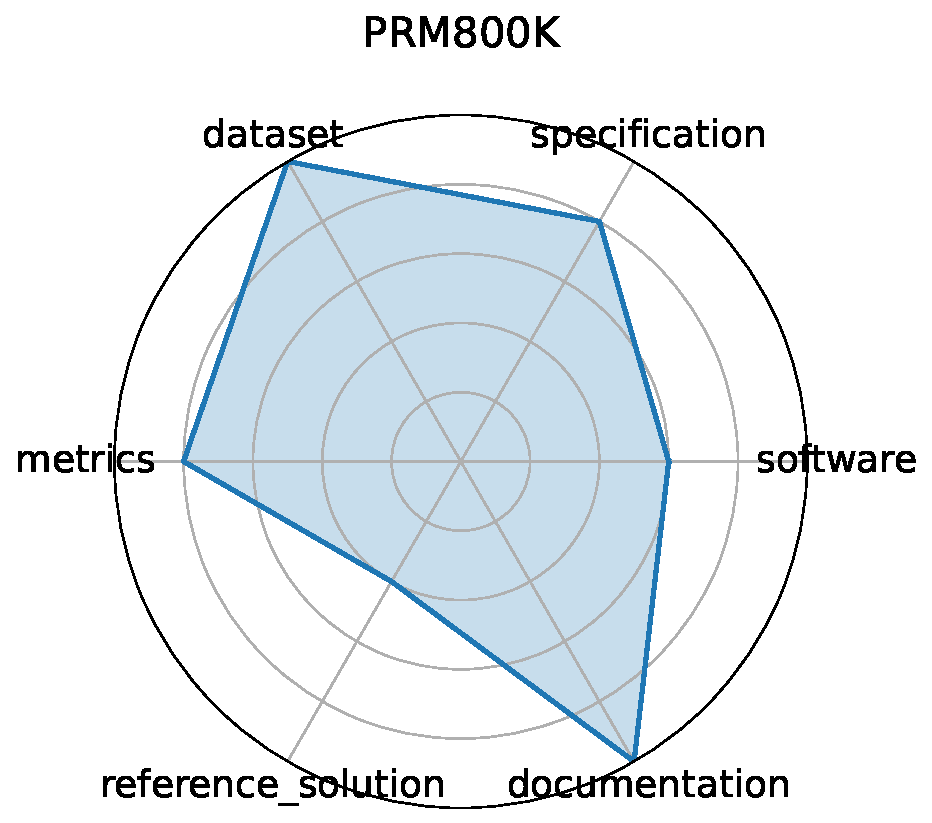
\includegraphics[width=0.2\textwidth]{prmk_radar.pdf}
}}
\clearpage